%!TEX root = ../thesis_polimi.tex

\chapter{Introducing Cerberus} % (fold)
\label{chap:approach}

\start{C}{erberus} or Kerberos (Κέρβερος) is a three-headed guardian dog from the Greek mythology, in charge of
patrolling the gates of Hades, land of the dead. Preventing dead souls to evade the
underworld was his duty. In the same fashion we wanted to build a tool to \emph{detect}
malicious domains employed by botnets and track down the IP addresses these domains resolve
to, as to guarantee that they shall not tarnish the namespace ever again.

As the hellhound featured three heads, our \thesystem operates in three
phases: The \important{Bootstrap Phase}, where the initial optional ground truth is
generated, the \important{Filtering Phase}, where the DNS data is filtered, and the
\important{Detection Phase}, where domains are classified and new threats are
discovered.

\paragraph{Chapter Organization} The remainder of this chapter is organized in the
following fashion:
\begin{itemize}
    \item in Section~\ref{sec:approach_overview} we will describe \thesystem at
        a high level of abstraction, providing an overview of the overall process;
    \item in Section~\ref{sec:approach_details} we will tackle all the
        elements that form \thesystem.
\end{itemize}

\newpage

\section{Cerberus Overview} % (fold)
\label{sec:approach_overview}
\sectionstart{C}{erberus} is composed of three main modules or phases: \important{Bootstrap},
\important{Filtering} and \important{Detection} (see Figure~\ref{fig:cerberus_overview_approach}). The \important{Bootstrap Phase} is fed with a blacklist of malicious domains and
provides the initial ground truth to the system in an automatic and unsupervised fashion. We use the term \emph{ground truth} to refer to the knowledge that the
system trusts even though its correctness was not validated by any external authority.
The ground truth consists of a set of clusters of domain names and the IP addresses they
resolve to, clusters that represent DGA-based malicious activities employing the same DGA.
This knowledge is used by the \important{Detection Phase}.

\begin{figure}[!htp]
    \centering
    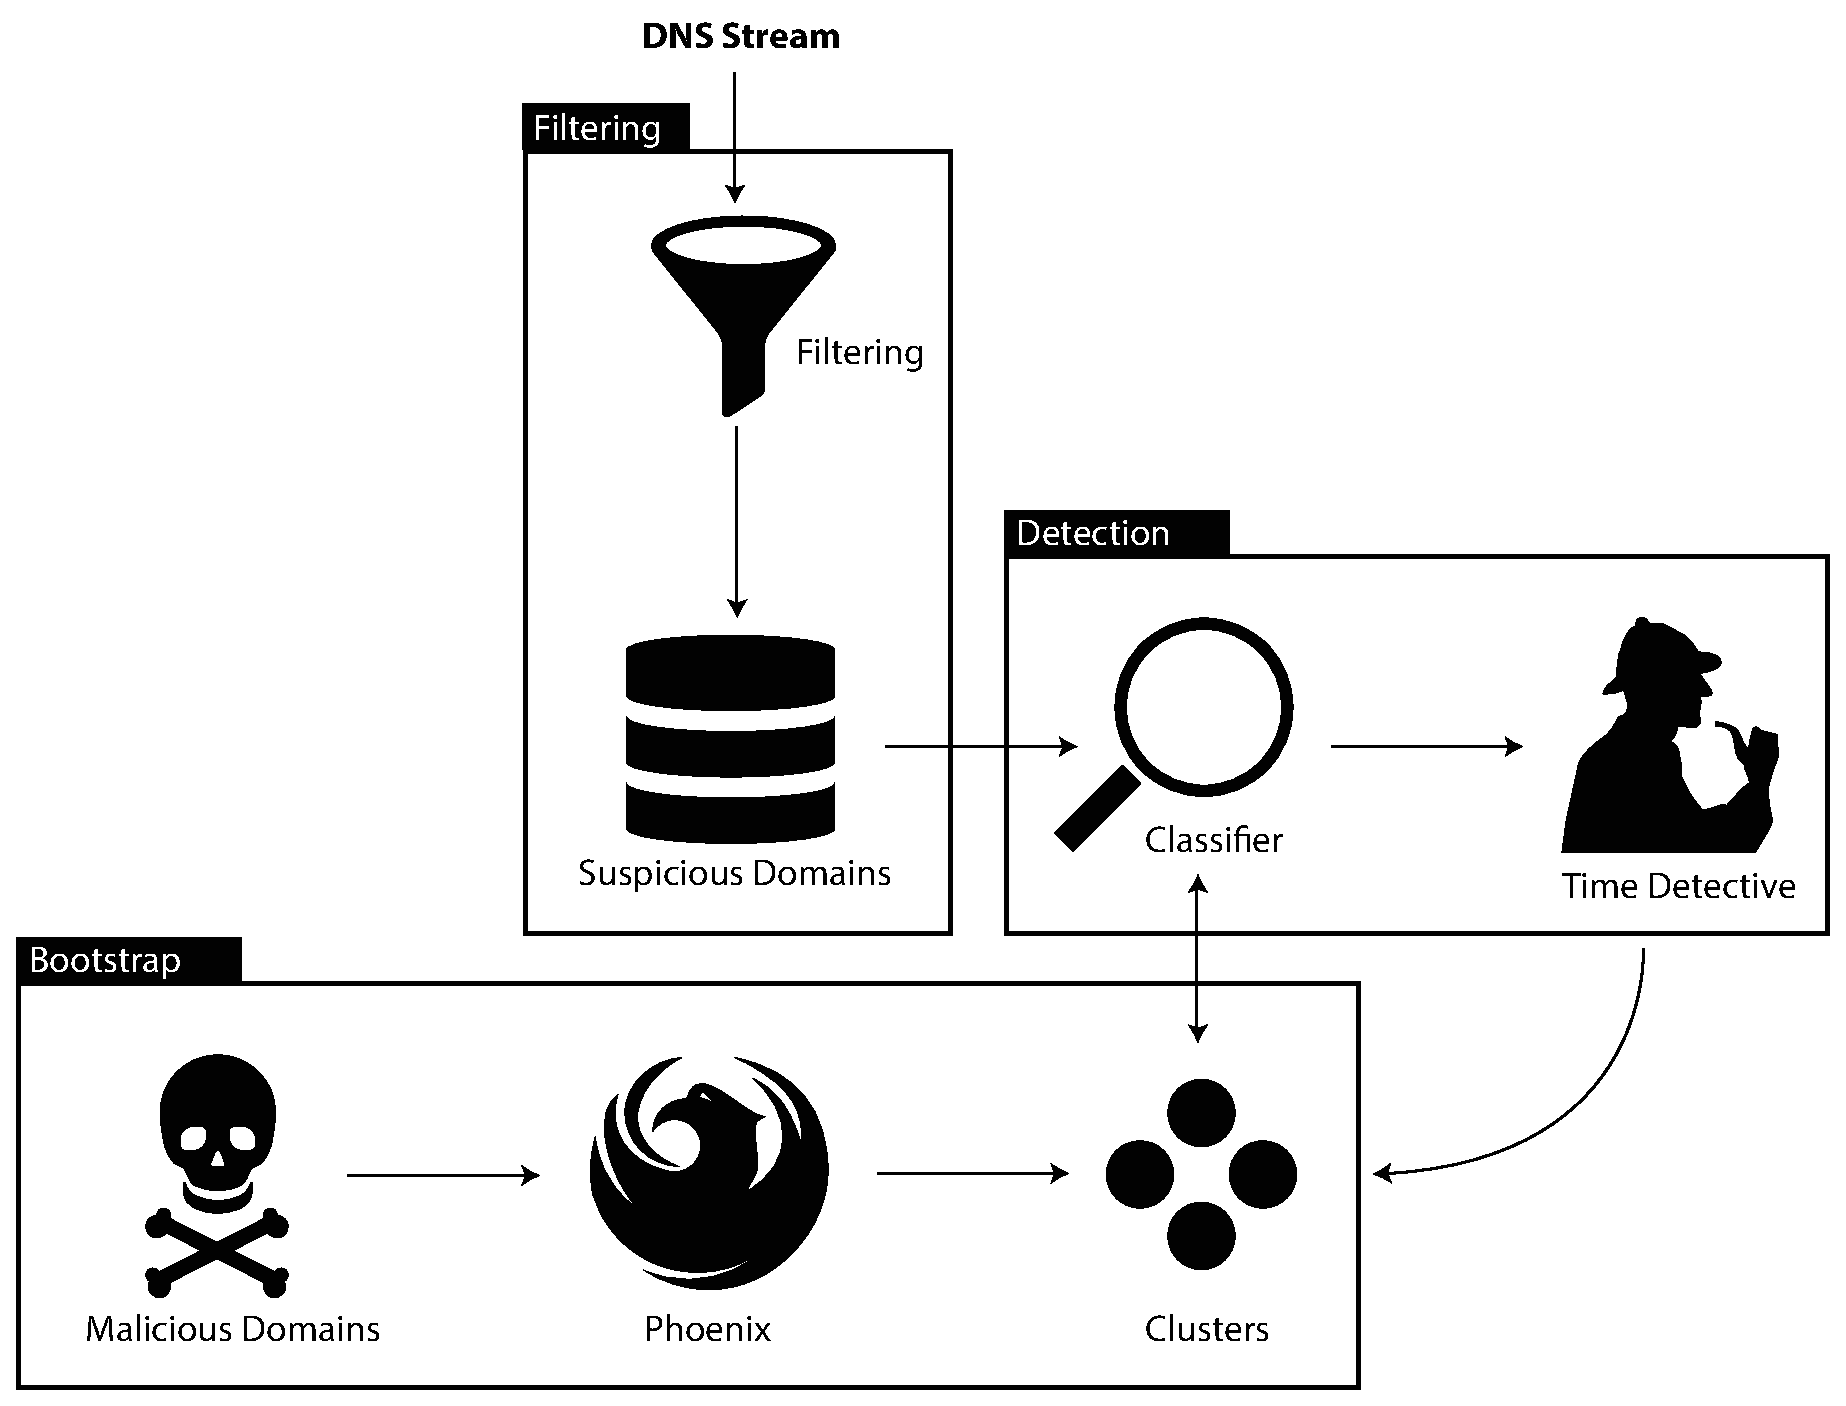
\includegraphics[width=\linewidth]{cerberus.eps}
    \caption{Cerberus overview.}
    \label{fig:cerberus_overview_approach}
\end{figure}

The \important{Detection Phase} consumes the output of the \important{Filtering Phase}, where a stream of
DNS replies is filtered to obtain a list of likely malicious domains. To this end
we employ a list of filters mostly based on heuristics and whitelists to reduce as
much as possible the number of legitimate domains, while keeping the suspicious
ones.
After the \important{Filtering Phase} is completed, the Classifier uses the
ground truth previously generated to \emph{detect} known threats, i.e., the Classifier returns a list of malicious domains labeled with one of the clusters from the ground truth. To this end,
for each unseen domain it selects those clusters that share the domain IP address
and then decides to which one  it should be assigned using a Support Vector Machine that leverages the Subsequence String Kernel to compute similarity between strings.

Those domains that do not share their IP address with the ground truth are fed to
the \textbf{Time Detective}: The rationale is that at this very moment we cannot establish whether these ``suspicious'' domains are actually malicious, but by analyzing the activity related to their IP addresses we may be able to correctly identify the threats. The \textbf{Time Detective} stores the ``suspicious'' IP addresses
and keeps track of the domains that resolve to them throughout time. After $\Delta$ time has passed it groups them by their Autonomous System,
and clusters together the domains that are deemed similar (see Section~\ref{par:dbscan_clustering}).
After the new clusters are generated they are added to the ground truth and this
further knowledge is then used to increase the range of detected threats.

\begin{figure}[!htp]
    \centering
    \begin{tikzpicture}
        \node (DETECTION) {Detection};
        \node[above left=1cm of DETECTION] (BOOTSTRAP) {Bootstrap};
        \node[below right=of DETECTION,minimum height=3em] (CLUSTERING) {Clustering};
        \node[below left=of DETECTION, align=center, minimum height=3em] %
            (KNOWLEDGE) {Increase\\Knowledge};
        \node[below=3.3cm of DETECTION] (DISCOVER) {Discover};

        \node [right=0cm of CLUSTERING]  {
\includegraphics[width=.6cm]{detective.eps}};
        \node [below=0cm of DETECTION]  {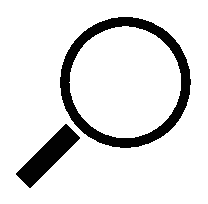
\includegraphics[width=.6cm]{classifier.eps}};
        \node [left=0cm of BOOTSTRAP]  {
\includegraphics[width=.6cm]{phoenix.eps}};
        \node [left=0cm of KNOWLEDGE]  {
\includegraphics[width=.6cm]{knowledge.eps}};

        \path[arrow]
            (BOOTSTRAP.east)  edge[bend left] (DETECTION.north)
            (DETECTION)  edge[bend left]  (CLUSTERING)
            (CLUSTERING) edge[bend left] (DISCOVER)
            (DISCOVER)   edge[bend left] (KNOWLEDGE)
            (KNOWLEDGE)  edge[bend left] (DETECTION)
        ;
    \end{tikzpicture}
    \caption{Cerberus lifecycle.}
    \label{fig:cerberus_lifecycle}
\end{figure}

This process is summarized in Figure~\ref{fig:cerberus_lifecycle}: \thesystem can automatically evolve by increasing its
knowledge in an unsupervised fashion: The Clustering routine allows to discover
new threats that are added to the ground truth. Then the system can return in
the \important{Detection Phase}, leveraging the new knowledge.
In the next section we discuss in further detail what briefly described above.
The symbols used in Figure~\ref{fig:cerberus_overview_approach} will provide a visual aid
to better understand which part of the schema we will be describing.
% section approach_overview (end)

\newpage

\section{Cerberus Details} % (fold)
\label{sec:approach_details}
\sectionstart{I}{n} the previous section we have given a brief overview of how
\thesystem works. In the following of this section, we shall go in deeper detail,
throughly explaining every aspect of the \important{Bootstrap}, \important{Filtering}
and \important{Detection} phases.

\subsection{The Bootstrap Phase} % (fold)
\label{sub:the_bootstrap_approach}
\begin{wrapfigure}{l}{2.2cm}
\centering
    
\includegraphics[width=2cm]{phoenix.eps}
\end{wrapfigure}
The \important{Bootstrap Phase} aims at providing \thesystem with the initial ground
truth. This knowledge is not mandatory to have, as the system needs no \emph{a
priori} knowledge to start detecting new threats. Nevertheless it is useful to have
the possibility to plug it into \thesystem, which can use it to label the unseen domains during the \important{Detection Phase}. To this end we employ
\phoenix. \phoenix takes as initial input a list of malicious domains. It then
applies a DGA filter (the same used in Paragraph~\ref{par:phoenix_dga_filter})
to filter out those domains that appear likely benign, under the assumption that domains generated manually, by a human, are benign, in contrast to AGDs, which are generated automatically by a DGA. Therefore
the remaining domains are both \emph{non-benign} (i.e., suspicious) and \emph{automatically generated}.

\thesystem clusters these domains depending on the IP address(es) they resolve to. Hence
at the end of the clustering process, \thesystem has a list of clusters of domains
and the IP addresses they resolve to, domains produced by the same DGA and IP
addresses that should belong to the C\&C servers, and it will later leverage this
list to label unseen domains in the \important{Detection Phase}.

\dataexample{%
    \parbox{.9\textwidth}{
    The following are two of the eleven clusters generated by the
    \important{Bootstrap Phase}:}
    \vspace{.1cm}
    \begin{center}
    \begin{minipage}{.5\textwidth}
            \centering
            \begin{tabular}{rp{2.8cm}}
            \multicolumn{2}{l}{\textsc{Cluster f105c}} \\
            \midrule
            Threat: & Palevo \\
            IPs: & \texttt{176.74.176.175} \newline \texttt{208.87.35.107} \newline \newline \\
            Domains: & \texttt{cvq.com} \newline \texttt{epu.org} \newline \texttt{bwn.org} \\
            \end{tabular}
        \end{minipage}%
        \begin{minipage}{.5\textwidth}
            \centering
            \begin{tabular}{rp{2.8cm}}
                \multicolumn{2}{l}{\textsc{Cluster 0f468}} \\
                \midrule
                Threat: & Sality \\
                IPs: & \texttt{217.119.57.22} \newline \texttt{91.215.158.57} \newline \texttt{178.162.164.24} \newline \texttt{94.103.151.195} \\
                Domains: & \texttt{jhhfghf7.tk} \newline \texttt{faukiijjj25.tk} \newline \texttt{pvgvy.tk} \\
            \end{tabular}
        \end{minipage}
    \end{center}
}

% subsection the_bootstrap (end)

\subsection{The Filtering Phase} % (fold)
\label{sub:the_filtering_phase}
\begin{wrapfigure}{l}{2.2cm}
\centering
    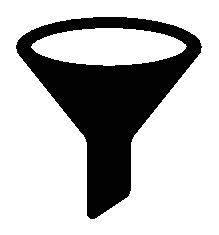
\includegraphics[width=2cm]{filter.eps}
\end{wrapfigure}
After the \important{Bootstrap Phase}, \thesystem aims at classifying unseen
domains from a stream of DNS passive data.
The DNS stream we receive comes from the real world, hence it features both benign and malicious
domains. Therefore we want to reduce as much as we can the amount of legitimate domains
while keeping as many malicious domains as possible. To achieve this goal the DNS feed goes
through a list of filters listed here below.

\paragraph{Alexa Whitelist} % (fold)
\label{par:alexa_whitelist}
This filter removes all the domains that rank amongst the first 1,000,000 in the Alexa Top
Domains list. The rationale is that the most popular domains in the Web are less likely to be malicious.
Even though this is not completely true (as of 2012, BarracudaLabs found 58 drive-by-download
malicious websites in the first 25,000 Alexa domains\footnote{\url{https://media.blackhat.com/ad-12/Royal/bh-ad-12-quanitfying-royal-slide.pdf}}), there are no known cases of malicious AGDs found among the Alexa Top 1M. Moreover we are looking for domains
used to set up the C\&C channel: They are usually valid for one day and then thrown away and
it is very unlikely that they make it to the list.
% paragraph alexa_whitelist (end)

\paragraph{Content Distribution Networks} % (fold)
\label{par:content_distribution_networks}
DGAs are used to legitimate ends by Content Delivery Networks (CDNs). These
infrastructures consist of a large distributed system of servers, deployed with the
intention of providing users with content at high availability and high performance.
YouTube and Amazon CloudFront are examples of this type of networks. In our system we
filled in a list of the most popular CDNs: If a domain belongs to one of them it is
filtered out. For instance, the domain \texttt{r4---sn-a5m7lnes.c.youtube.com}
belongs to the YouTube CDN: It was clearly generated by some DGA, but it is not
malicious and therefore it must be filtered out.
% paragraph content_distribution_networks (end)

\paragraph{Top Level Domain Whitelist} % (fold)
\label{par:top_level_domain_whitelist}

Some TLDs require clearance before the domain can be registered (see Table~\ref{tab:tlds_clearance}). When the attackers register their domains they do not want to go through authorizations
by third party authorities, for two obvious reasons: \emph{i)} they do not want anyone to
investigate the domain they are going to register and \emph{ii)} they cannot wait for the time required by
clearance process. Therefore all of those domains that feature a TLD listed in Table~\ref{tab:tlds_clearance} are filtered out.

\begin{table}[!htp]
    \centering
    \begin{tabular}{rp{4cm}rp{4cm}}
        \toprule
        \textsc{TLD} & \textsc{Entity} & \textsc{TLD} & \textsc{Entity} \\
        \midrule
        \texttt{.ac.uk} & British academic\newline domains & \texttt{.edu} & educational \\
        \texttt{.aero} & air-transport industry   & \texttt{.gov} & governmental \\
        \texttt{.arpa} & Address and Routing \newline Parameter Area & \texttt{.int} & international \newline organizations \\
        \texttt{.coop} & cooperatives & \texttt{.mil} & US Military \\
        \texttt{.museum} & museums & \texttt{.pro} & professions \\
        \texttt{.post} & postal services & \texttt{.travel} & travel and tourism \newline industry \\
        \bottomrule
    \end{tabular}
    \caption{TLDs requiring clearance before registration.}
    \label{tab:tlds_clearance}
\end{table}
% paragraph top_level_domain_whitelist (end)

\paragraph{Time To Live} % (fold)
\label{par:time_to_live}
The TTL parameter sets for how long a cached DNS record is to be considered valid in a local
DNS Server. Previous works in literature (\cite{bilge2011exposure}, \cite{holz2008})
stated that this value was set to very low values (100s) in the case of malicious
domains. The rationale, from the botnet operators, is that these infrastructures need to update fast their C\&C locations and therefore need the DNS server to update the records at the same pace. However, more recent investigations seem to state the
opposite. \citet{xu2013} from Palo Alto Networks reported that approximately 80\%
of fast-flux domains exhibit a change rate greater than 30 minutes/IP, while in
2008 \citet{holz2008} reported that fast-flux domains
exhibited a changing rate less than 10 minutes/IP. This change, and the subsequent
change in TTL values, is due economic reasons and to avoid detection based on
changing rate. Therefore we decided to filter out all the domains featuring a low
TTL value, less than 300 seconds. We chose this value after analyzing two weeks
of DNS data from the ISC/SIE dataset in our possession: We manually searched for
the domains classified as malicious by an early version of \thesystem, and noticed
that all the benign domains featured a TTL equal or lower than 300 seconds.
% paragraph time_to_live (end)

\paragraph{\phoenix DGA Filter} % (fold)
\label{par:phoenix_dga_filter}
The domains employed in DGA-based malicious activities feature that randomness captured
by \citet{schiavoni2013} in \phoenix. Therefore we filter out those domains that do
not exhibit the required level of randomness to be labeled as AGDs.
% paragraph phoenix_dga_filter (end)

\paragraph{Whois Queries} % (fold)
\label{par:whois_queries}
Finally we look at the registration date. We leverage the insight that attackers
do not (and sometimes \emph{cannot}, as when using unpredictable seed in the DGA, e.g., Twitter trend topic) register
their domains much time in advance, as otherwise they would
not be able to leverage the resilient migration strategy allowed by the use of DGAs:
If the C\&C is unveiled they should update the DNS records for all the
pre-registered domains.

Therefore we query a \texttt{Whois} server to ask for the registration date of every domain:
If the domain is ``old'' it is discarded, whereas if either it was recently registered or
the \texttt{Whois} server replied with an error code (e.g., no information is available for that domain), we conservatively keep the domain. For all the
retained domains we
store the registration date for later use in the detection phase.
% paragraph whois_queries (end)

\paragraph{Summary} % (fold)
\label{par:summary}
We want to recap here the features of the domains that remain at the end of the
filtering process and that constitute the input for the \important{Detection Module}.
For each step we report also the number of domains that persist after the filtering
process in a pilot experiment conducted on 30' of sampled traffic (see Section~\ref{sec:dataset}).


\begin{description}[labelwidth=\widthof{20,000}, leftmargin=!, align=parright]
    \item[20,000] domains remain with a TTL greater than 300 seconds;
    \item[19,000] domains not in the Alexa Top 1M whitelist;
    \item[15,000] domains not in the most popular CDNs;
    \item[800] domains likely to be AGDs;
    \item[700] domains featuring a TLD that does not require previous authorization;
    \item[300] domains that have been recently registered.
\end{description}

% paragraph summary (end)

% subsection the_filtering_phase (end)

\subsection{The Detection Phase} % (fold)
\label{sub:dga_detection}
In the \important{Detection Phase}, we aim at recognizing domains belonging to known botnets
and to discover new ones. These two tasks are achieved by two different modules: The
\important{SSK Classifier} and the \important{Time Detective} respectively.

\subsubsection{The Subsequence String Kernel Classifier} % (fold)
\label{ssub:ssk_classifier}
\begin{wrapfigure}{l}{2.2cm}
\centering
    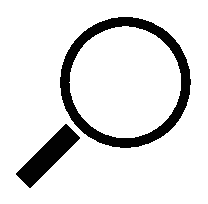
\includegraphics[width=2cm]{classifier.eps}
\end{wrapfigure}
This component is fed with the data coming from the \important{Filtering Phase}.
It classifies each unseen domain domain $d$ using the knowledge provided
by \phoenix, i.e., the clusters of DGAs, eventually including those generated by \thesystem. The classifying process consists of assigning
$d$ to one of those clusters.
\citet{schiavoni2013} had developed their own classifier, but it suffered from the major
shortcoming of using \emph{ad hoc} parameters, such as the domain length and the TLD.
This means that if $d$ features a TLD other than those in the clusters, or if it
features a length that does not reside in the previously seen boundaries, it is discarded.

We wanted to have a classifier resilient to such changes, one that would label $d$ leveraging
only the \emph{string} itself as a feature to compute similarity amongst $d$ and the clusters.
\citet{haddadi2013malicious} compared different approaches in classifying AGDs: As the Support
Vector Machine technique outplayed all the others with respect to the F-Score,
we decided to use this approach.

\paragraph{Support Vector Machines} % (fold)
\label{par:support_vector_machines}
The Support Vector Machine is a binary learning machine that can be used for classification
and rule regression~\cite{alpaydin2004introduction}. The main idea of this classification
algorithm is to build a hyperplane that optimally separates the samples of data into two
categories with maximal margin~\cite{haddadi2013malicious}. It is possible to build a
\emph{k}-classes classifier, with $k$ greater than two, by building $k$ binary classifiers.

Support Vector Machines must undergo a \emph{training phase}, where they are fed with points
in the form of $\{\vec{x_i}, y_i\}$, where $\vec{x_i}$ is a feature vector and $y_i$ is the
binary class label (e.g., $1$ or $-1$). Note that in our context, the labels need not to be provided manually because we use clusters as labels, which are generated automatically. There is a parameter to be set during the classification process:
$C$, which controls the punishment function for misclassified points. In our implementation
we left this parameter to 1, its default value.

When dealing with linear data we have to
find two hyperplanes:
\[ \vec{w} \cdot \vec{x} -b = 1\]
\begin{center}
and
\end{center}
\[ \vec{w} \cdot \vec{x} -b = -1\]
that bound a region, called \emph{the margin}, where no data point is present. Training the
SVM in this case means to maximize the distance between the hyperplanes.
SVMs can be also employed to classify data that are non-linearly separable, but they need to
be equipped with a \emph{kernel function}, a non-linear mapping of an input data into a high
dimensional feature space~\cite{haddadi2013malicious}. When the mapping is completed, the
hyperplane that maximizes the separation margin can be constructed. Then, as a final step,
a linear mapping from the feature space to the output space is required~\cite{haddadi2013malicious}. In the next paragraph we shall better explain what a kernel function
is and introduce the Subsequence String Kernel.

% paragraph support_vector_machines (end)

\paragraph{Subsequence String Kernel} % (fold)
\label{par:subsequence_string_kernel}
A function that calculates the inner product between mapped examples in a feature space
is a kernel function~\cite{lodhi2002}. Therefore for any mapping:
\[ \phi \; : \; D \rightarrow F \]
we define a kernel function as
\[ K(d_i, d_j) = \langle \phi(d_i), \phi(d_j) \rangle \]
where $\langle \cdot , \cdot \rangle$ is the dot product and $d_i$, $d_j$ are feature vectors.
In 2002 \citet{lodhi2002} proposed a kernel function to measure the similarity of strings.
The idea is to compare them by means of the substrings they contain: The more substrings
in common, the more similar they are~\cite{lodhi2002}. We can better explain the process
by looking at the example in Table~\ref{tab:SSK}.

\begin{table}[!htp]
    \begin{minipage}{.5\textwidth}
    \begin{tabular}{lacccc}
                        & c-a         & c-t         & a-t         & c-r          & a-r         \\
        \midrule
        $\phi($cat$)$   & $\lambda^2$ & $\lambda^3$ & $\lambda^2$ &  0           & 0           \\
        $\phi($car$)$   & $\lambda^2$ & 0           & 0           &  $\lambda^2$ & $\lambda^2$ \\
    \end{tabular}
    \end{minipage}%
    \begin{minipage}{.5\textwidth}
        \begin{align*}
        \text{ker}(car,cat) &= \lambda^4 \\
        \text{ker}(car,car) &= \text{ker}(cat,cat) = 2\lambda^4 + \lambda^6 \\
        \text{ker}(car,cat) &= \frac{\lambda^4}{(2\lambda^4 + \lambda^6)} = \frac{1}{(2 + \lambda^2)}
    \end{align*}
    \end{minipage}
    \caption{SSK example from \citet{lodhi2002}.}
    \label{tab:SSK}
\end{table}

We consider the two strings \texttt{car} and \texttt{cat}. The first step is to compute the feature space of the strings to be compared.
In this case it is a 5-dimensions space composed by the features \texttt{c-a}, \texttt{c-t},
\texttt{a-t}, \texttt{c-r} and \texttt{a-r}, which are all the possible non-contiguous
 two characters long substrings of \texttt{car} and \texttt{cat}.

We then set a \emph{decay factor} $\lambda$ that measures a decay in the quality of the
similarity between strings, i.e., if we have $\lambda^n$, it means that we need $n$
characters of the string to match the substring. In our example we have for instance
\texttt{c-t}, which is present in \texttt{cat}, but it requires three characters to be
matched: \important{c}, a and \important{t}. That is why we then find $\lambda^3$ in the
cell ($\phi(\text{cat})$, \texttt{c-t}).

We then define the inner product between two strings $s$ and $t$ as the sum over all common
subsequences weighted according to their frequency of occurrence and lengths~\cite{lodhi2002}.
In formulas:

\[ %
    K_n(s,t) = \sum_{u \in \sum^n} \langle \phi_u(s) \cdot \phi_u(t) \rangle %
             = \sum_{u \in \sum^n} \sum_{\vec{i}:u=s[\vec{i}]} \sum_{\vec{j}:u=t[\vec{j}]} %
                \lambda^{l(\vec{i})+l(\vec{j})} %
\]
In our example \texttt{car} and \texttt{cat} share only the substring \texttt{c-a}
(we have highlighted the column). Therefore we have:
\[ \text{ker}(car,cat) = \lambda^2 + \lambda^2 = \lambda^4 \]
which is the unnormalised kernel. To get the normalised kernel we divide by
$\text{ker}(car,car) = \text{ker}(cat,cat) = 2\lambda^4 + \lambda^6$, which
yields $\frac{1}{(2 + \lambda^2)}$.
% paragraph subsequence_string_kernel (end)

\paragraph{The Classification Process} % (fold)
\label{par:the_classification_process}
When an unseen domain $d$ arrives, we select the clusters that share the IP address with $d$.
Those clusters are used to train the Support Vector Machine that is then used to classify
$d$. What happens when no cluster shares the IP address with $d$ is explained in the
next paragraphs.
% paragraph the_classification_process (end)
% subsubsection ssk_classifier (end)

\subsubsection{The Time Detective} % (fold)
\label{ssub:the_time_detective}
\begin{wrapfigure}{l}{2.2cm}
\centering
    
\includegraphics[width=2cm]{detective.eps}
\end{wrapfigure}
When an unseen domain $d$ does not share the IP address with the clusters of the ground
truth, we issue the
\important{Time Detective}: We want to keep track of the activity related to its IP address for $\Delta$ time to see if it shows hints of maliciousness.

After
$\Delta$ time has passed, first we group together domains that resolved to IPs that
reside in the same Autonomous Systems, then we try to extract clusters of similar (similarity is computed using the SSK) domains using the DBSCAN
clustering algorithm. After the clustering routine is done, we add these new clusters of malicious domains to the ground truth. To see whether two clusters (one from the new ones and the
other from the old ones) are similar, we run a similarity test. After this
stage is completed, \thesystem starts classifying new unseen domains, leveraging
the increased knowledge.
In the next paragraphs we shall tackle every aspect of the aforementioned process.

\paragraph{DBSCAN Clustering} % (fold)
\label{par:dbscan_clustering}

The DBSCAN algorithm relies on the concept of \emph{density reachability}. In
Figure~\ref{fig:dbscan} $B$ is density-reachable by $A$, as there is a chain of data points
such that the next point is no farther from the previous one than $\varepsilon$.
DBSCAN allows several metrics to measure the distance among samples: Euclidean, Manhatthan, Jaccard and Mahalanobis are a few examples. In \thesystem we use a
Kernel Distance and we compute the distance matrix using the Subsequence String
Kernel.
$\varepsilon$ is a parameter set \emph{a priori}, usually by looking at the k-distance graph.
The other parameter DBSCAN requires to be set is \emph{minPts}, the minimum number of points required to
form a cluster. For instance, in our situation, if \emph{minPts} was set to four, all the
points from $A$ to $B$ would belong to the same cluster. If it was set to six, all the
points from $A$ to $B$ would be considered noise.
\begin{figure}[!htp]
    \centering
    \begin{tikzpicture}
        \node[dbscan] (CIRCLE) {\tikz \node[dbscan_circle] (DOT) {}; };
        \node[below=0 cm of DOT.south, anchor=north] {A};
        \dbnode{1}{2}{A}{B}
        \dbnode{1.5}{2.7}{C}{D}
        \node at (1.1,2.7) {B};
        \dbnode{2}{1.3}{E}{F}
        \dbnode{1.2}{0.5}{G}{H}
        \dbnode{3.9}{1.1}{I}{L}
        \node at(3.9,0.6) {noise};
        \path[arrow]
            (DOT) edge node[left] {$\varepsilon$} (CIRCLE)
            ;
        \path[arrow, ultra thick, BrickRed]
            (1,2) edge (1.5,2.7)
            (2,1.3) edge (1,2)
            (1.2,0.5) edge (2,1.3)
            (DOT) edge (1.2,0.5)
            ;
    \end{tikzpicture}
    \caption{The DBSCAN Algorithm.}
    \label{fig:dbscan}
\end{figure}
In our implementation we set the \emph{minPts} parameter to $\Delta$, where $\Delta$ measures in days how much time we wait before performing the clustering routine. We chose this number
following this rationale: In $\Delta$ time a cluster must count at least one domain
for each day passed, i.e., the bots must have contacted the C\&C Server at least once a day.
In the next paragraph we will explain how we set the $\varepsilon$ parameter.
% paragraph dbscan_clustering (end)

\paragraph{$\varepsilon$ estimation} % (fold)
\label{par:paragraph_name}
To estimate $\varepsilon$ we used a heuristic that leverages the \emph{k distance} graph.
The \emph{k distance} graph is a graph in which two vertices $p$ and $q$ are connected by an
edge, if the distance between $p$ and $q$ is among the $k$-th smallest distances from
$p$ to other objects of the population\footnote{\url{https://en.wikipedia.org/wiki/Nearest_neighbor_graph}}. We set $k$ equal to \emph{minPts}, and we calculate the
variance of the distances for the neighborhood of each point. We then consider the point that
features the neighborhood with the lowest variance. From that neighborhood we take the
highest distance. The rationale is that we want to be sure that the \emph{minPts} least
dispersed points are clustered together.

It could happen that this value needs to be slightly adjusted. Therefore we modify $\varepsilon$
using a tolerance $\tau$ parameter. In formulas:
\[ \varepsilon = \varepsilon \times \tau \]
We try different values of $\tau$ that range from -0.5 to 0.5, step 0.1, and we choose the value
that yields the best clustering quality. In the next paragraph we explain how we measure
the clustering quality.

% paragraph paragraph_name (end)

\paragraph{Measuring Clustering Quality} % (fold)
\label{par:measuring_clustering_quality}
To measure the clustering quality we use the C-Index proposed by \citet{hubert1976}.
They define $N_W$ as the sum of the number of pairs in each cluster:
\[ N_W = \sum^K_{k=1} \frac{n_k(n_k-1)}{2} \]
where $n_k$ is the cardinality of cluster $k$.
They then define $S_W$ as the sum of the $N_W$ distances between all the pairs of points
inside each cluster, $S_{\mathrm{min}}$ as the sum of the $N_W$ smallest distances between all
the pairs of points in the entire dataset and $S_{\mathrm{max}}$ as the sum of the $N_W$ largest
distances between all the pairs of points in the entire dataset.

\citet{hubert1976} define the C-Index as the ratio of the sum of distances infra-cluster to the sum
of the distances intra-clusters (normalized). The C-Index ranges from 0 to 1, and lower
values yield better clusters.
In formulas:
\[ C = \frac{S_W - S_{\mathrm{min}}} {S_{\mathrm{max}} - S_{\mathrm{min}}} \]

As previously stated we iterate the clustering process for each list of domains over eleven
values of tolerance (from -0.5 to 0.5, step 0.1) and keep the clusters that
feature the lowest C-Index. Once the process is completed for all the Autonomous Systems,
we have to decide whether the new clusters must be \emph{added} to the ground truth
produced by \phoenix, or if there are couples of clusters that, though not sharing the
IP addresses, should be \emph{merged} together as they represent the same family of DGA.
In the next paragraph we explain how we measure similarity between clusters.

\dataexample{%
During the test described in Section~\ref{sec:cerberus_in_the_wild}, When applying the clustering routine to AS 22489,
$$\tau= 0.2$$
yielded the lowest value of $\text{C-Index}= 0.0032$.
}
% paragraph measuring_clustering_quality (end)

\paragraph{Measuring Clusters Similarity} % (fold)
\label{par:measuring_clusters_similarity}
\thesystem is able to tell when two clusters are to be merged together. To this
end it employs the Welch's test.

Suppose we want to establish whether cluster $A$ should be merged or not with
cluster $B$. We can represent both of the clusters in matrix form, where we have
the elements on rows and columns, and a cell contains the \emph{distance} between
the elements, computed using the SSK.

\[
A_{m,m} =
\bordermatrix{
         & a_1     & a_2     & \cdots & a_m     \cr
  a_1    & a_{1,1} & a_{1,2} & \cdots & a_{1,m} \cr
  a_2    & a_{2,1} & a_{2,2} & \cdots & a_{2,m} \cr
  \vdots & \vdots  & \vdots  & \ddots & \vdots  \cr
  a_m    & a_{m,1} & a_{m,2} & \cdots & a_{m,m}}
 \quad
 B_{n,n} =
 \bordermatrix{
         & b_1     &  \cdots & b_n     \cr
  b_1    & b_{1,1} &  \cdots & b_{1,n} \cr
  b_2    & b_{2,1} &  \cdots & b_{2,n} \cr
  \vdots & \vdots  &  \ddots & \vdots  \cr
  b_n    & b_{n,1} & \cdots & b_{n,n}}
\]

We then build the $n \times m$ matrix $A \textasciitilde B$, which features the $n$
elements of $A$ as rows and the $m$ elements of $B$ as columns.
\[
 A \textasciitilde B_{m,n} =
 \bordermatrix{
         & b_1     & b_2     & \cdots & b_n     \cr
  a_1    & d_{1,1} & d_{1,2} & \cdots & d_{1,n} \cr
  a_2    & d_{2,1} & d_{2,2} & \cdots & d_{2,n} \cr
  \vdots & \vdots  & \vdots  & \ddots & \vdots  \cr
  a_m    & d_{m,1} & d_{m,2} & \cdots & d_{m,n}}
\]

We then run the Welch's test: The Welch's test is used when two samples may
show different variances and it is a variation of Student's \emph{t-test}.
We leverage the two-tailed test, where the null hypothesis states that the two
samples have equal mean. The test will yield a \emph{p-value} that will allow to
accept or reject the hypothesis. In \thesystem we decided to set the \emph{p-value}
to 1\%: Values greater than that will tell the clustering routine
that there is not enough statistical evidence to keep the clusters separated, and
\thesystem will merge the clusters together.

The rationale behind this procedure is that when two clusters actually are the same
cluster, if we mix the elements, the original cluster ($A$ in our example) and the
``mixed'' one ($A \textasciitilde B$) should feature the same distribution of
the distances.

\dataexample{%
Cluster \emph{a} and \emph{b} Welch's test yielded the values
$$t\simeq2.2 \quad \text{and} \quad p\simeq0.03$$
As we set the \emph{p-value} to 1\%, we cannot refuse $h_0$,
i.e., the clusters are merged together.
Further investigation on \url{palevotracker.abuse.ch} confirmed that both IP
sets identify Palevo C\&C (see Section~\ref{sec:cerberus_in_the_wild}).

\vspace{.2cm}

\begin{minipage}{.5\textwidth}
        \centering
        \begin{tabular}{lp{2.5cm}}
        \textsc{Cluster a} & \\
        \midrule
        IPs:           & \texttt{176.74.176.175} \newline \texttt{208.87.35.107} \newline \newline \newline \newline \\
        Domains & \texttt{cvq.com} \newline \texttt{epu.org} \newline \texttt{bwn.org} \\
        \end{tabular}
    \end{minipage}%
    \begin{minipage}{.5\textwidth}
        \centering
        \begin{tabular}{lp{2.5cm}}
            \textsc{Cluster b} & \\
            \midrule
            IPs: & \texttt{82.98.86.171} \newline \texttt{82.98.86.176} \newline
                \texttt{82.98.86.175} \newline \texttt{82.98.86.167} \newline \texttt{82.98.86.168} \newline \texttt{82.98.86.165} \\
            Domains & \texttt{knw.info} \newline \texttt{rrg.info} \newline
                \texttt{nhy.org} \\
        \end{tabular}
    \end{minipage}
}
% paragraph measuring_clusters_similarity (end)
% subsubsection the_time_detective (end)
% subsection dga_detection (end)
% section approach_details (end)

\section{Summary} % (fold)
\label{sec:approach_summary}
In this section we have introduced \thesystem and explained how it works.
\thesystem lifecycle is composed of three main phases. During the
\important{Bootstrap Phase} it produces the initial ground truth. When we
use the term \emph{ground truth}, we do not mean ground truth \emph{per se},
as there is no manual check of the results produced, but we mean the knowledge
that the system trusts. This knowledge is later used in the \important{Detection
Phase}, but before the actual detection can start \thesystem goes through
the \important{Filtering Phase}. During the filtering phase the DNS stream
to be analyzed is sifted out from legitimate domains, using a series of
heuristics. The remaining data is fed to the aforementioned
\important{Detection Phase}, during which \thesystem uses the clusters of AGDs from
the initial ground truth to label the unseen domains. Those domains that do not
share the IP address with the clusters are recorded for $\Delta$ time and then a clustering routine is performed. The newly generated knowledge is then added to
the system's ground truth.
In the next chapter we describe the implementation of \thesystem, focusing
on the crucial parts of the system.
% section summary (end)
% chapter approach (end)